% This file was created with tikzplotlib v0.10.1.
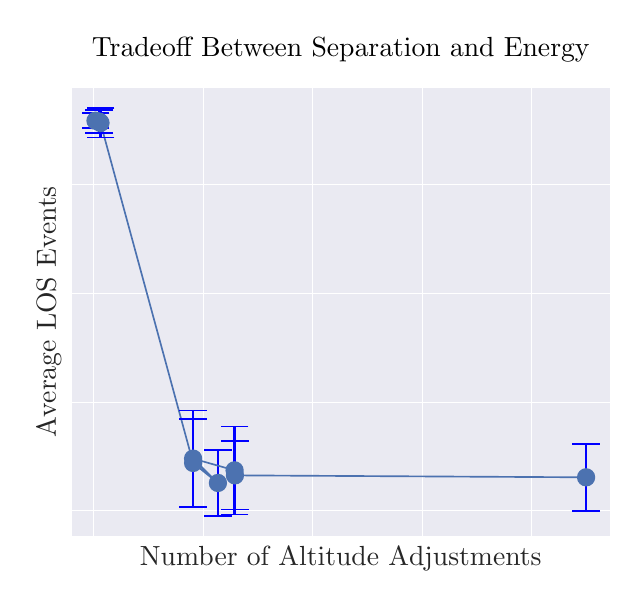
\begin{tikzpicture}

\definecolor{darkslategray38}{RGB}{38,38,38}
\definecolor{lavender234234242}{RGB}{234,234,242}
\definecolor{steelblue76114176}{RGB}{76,114,176}

\begin{axis}[
axis background/.style={fill=lavender234234242},
axis line style={white},
tick align=outside,
title={Tradeoff Between Separation and Energy},
x grid style={white},
xlabel=\textcolor{darkslategray38}{Number of Altitude Adjustments},
xmajorgrids,
xmajorticks=false,
xmin=-0.419606617647059, xmax=9.44423897058824,
xtick style={color=darkslategray38},
y grid style={white},
ylabel=\textcolor{darkslategray38}{Average LOS Events},
ymajorgrids,
ymajorticks=false,
ymin=-1.16772603652664, ymax=19.4513214113008,
ytick style={color=darkslategray38}
]
\path [draw=blue, thick]
(axis cs:8.99588235294118,-0.00544491975611994)
--(axis cs:8.99588235294118,3.08544491975612);

\path [draw=blue, thick]
(axis cs:2.57764705882353,0.0573907033213874)
--(axis cs:2.57764705882353,3.20260929667861);

\path [draw=blue, thick]
(axis cs:2.57102941176471,-0.164944443682345)
--(axis cs:2.57102941176471,3.88494444368235);

\path [draw=blue, thick]
(axis cs:1.81257352941176,0.190927796562548)
--(axis cs:1.81257352941176,4.60907220343745);

\path [draw=blue, thick]
(axis cs:2.26632352941176,-0.230496607079937)
--(axis cs:2.26632352941176,2.79049660707994);

\path [draw=blue, thick]
(axis cs:1.81308823529412,0.190024875775822)
--(axis cs:1.81308823529412,4.20997512422418);

\path [draw=blue, thick]
(axis cs:0.120073529411765,17.1659080181459)
--(axis cs:0.120073529411765,18.5140919818541);

\path [draw=blue, thick]
(axis cs:0.0980147058823529,17.3803847577293)
--(axis cs:0.0980147058823529,18.4196152422707);

\path [draw=blue, thick]
(axis cs:0.02875,17.5988255578154)
--(axis cs:0.02875,18.2811744421846);

\addplot [semithick, blue, mark=-, mark size=5, mark options={solid}, only marks]
table {%
8.99588235294118 -0.00544491975611994
2.57764705882353 0.0573907033213874
2.57102941176471 -0.164944443682345
1.81257352941176 0.190927796562548
2.26632352941176 -0.230496607079937
1.81308823529412 0.190024875775822
0.120073529411765 17.1659080181459
0.0980147058823529 17.3803847577293
0.02875 17.5988255578154
};
\addplot [semithick, blue, mark=-, mark size=5, mark options={solid}, only marks]
table {%
8.99588235294118 3.08544491975612
2.57764705882353 3.20260929667861
2.57102941176471 3.88494444368235
1.81257352941176 4.60907220343745
2.26632352941176 2.79049660707994
1.81308823529412 4.20997512422418
0.120073529411765 18.5140919818541
0.0980147058823529 18.4196152422707
0.02875 18.2811744421846
};
\addplot [semithick, steelblue76114176, mark=*, mark size=3, mark options={solid}]
table {%
8.99588235294118 1.54
2.57764705882353 1.63
2.57102941176471 1.86
1.81257352941176 2.4
2.26632352941176 1.28
1.81308823529412 2.2
0.120073529411765 17.84
0.0980147058823529 17.9
0.02875 17.94
};
\end{axis}

\end{tikzpicture}
